\documentclass{beamer}
\title{EMQX File Transfer II}
\author{Ilya Averyanov, Andrew Mayorov}
\institute{EMQX}
\date{2023}
\usetheme{emqx}
\usepackage{listings}
\usepackage{color}
\usepackage{graphicx}
\usepackage{xcolor}
\usepackage{hyperref}
\definecolor{href}{rgb}{0,0,0.9375}
\hypersetup{
    pdfborderstyle={/S/U/W 1}, % underline links instead of boxes
    colorlinks=true,
    urlcolor=href
}
\lstset{frame=tb,
  aboveskip=3mm,
  belowskip=3mm,
  showstringspaces=false,
  columns=flexible,
  basicstyle={\small\ttfamily},
  numbers=none,
  numberstyle=\tiny\color{gray},
  keywordstyle=\color{blue},
  commentstyle=\color{dkgreen},
  stringstyle=\color{mauve},
  breaklines=true,
  breakatwhitespace=false,
  tabsize=2
}


\begin{document}

\frame{\titlepage}

\begin{frame}
    \frametitle{File Transfer}
    \framesubtitle{Idea Recap}

    \begin{center}
        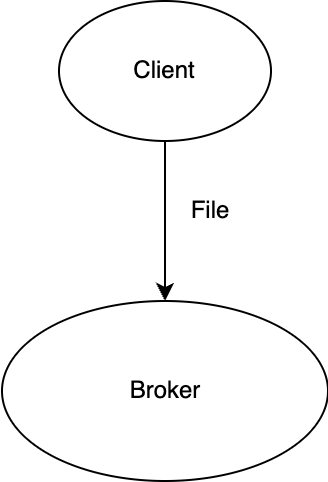
\includegraphics[height=5cm, keepaspectratio]{images/idea_naive.png}
    \end{center}
\end{frame}

\begin{frame}
    \frametitle{File Transfer}
    \framesubtitle{Constraints Recap}

    \begin{center}
        \begin{itemize}
            \item \href{https://github.com/emqx/eip/blob/main/active/0021-transfer-files-over-mqtt.md}{EIP 21}
            \item Over MQTT
            \item Chunked
            \item No additional connections from client
            \item No subcription to special topics
            \item Resumable
        \end{itemize}
    \end{center}
\end{frame}


\begin{frame}
    \frametitle{File Transfer}
    \framesubtitle{Idea}

    \begin{center}
        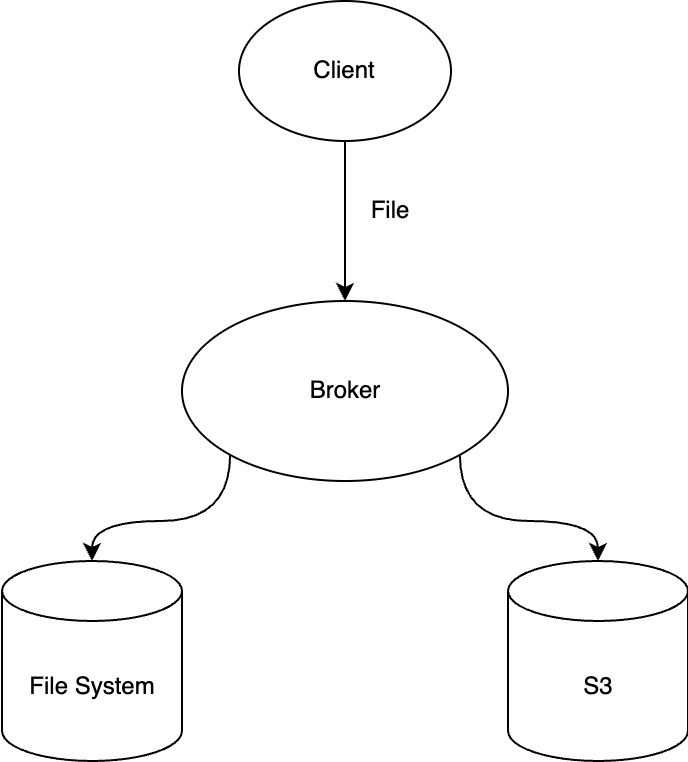
\includegraphics[height=5cm, keepaspectratio]{images/idea.png}
    \end{center}
\end{frame}


\begin{frame}
    \frametitle{File Transfer}
    \framesubtitle{emqx\_ft\_storage}

    \begin{center}
        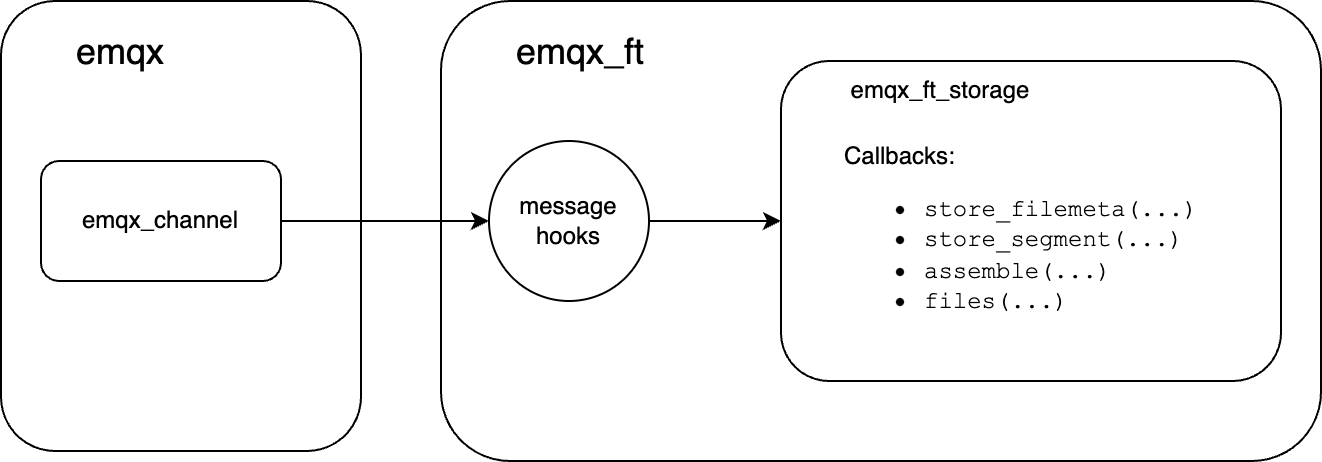
\includegraphics[width=9cm, keepaspectratio]{images/ft_storage.png}
    \end{center}
\end{frame}


\begin{frame}
    \frametitle{File Transfer}
    \framesubtitle{emqx\_ft\_storage\_fs}
    \begin{itemize}
        \item Keeps segments in the local file system
        \item Has segment assemble logic (from one or many nodes)
        \item Has segment GC logic
        \item Delegates file export to exporters
    \end{itemize}
    \begin{center}
    \end{center}
\end{frame}

\begin{frame}
    \frametitle{File Transfer}
    \framesubtitle{emqx\_ft\_storage\_fs config}

    \begin{center}
        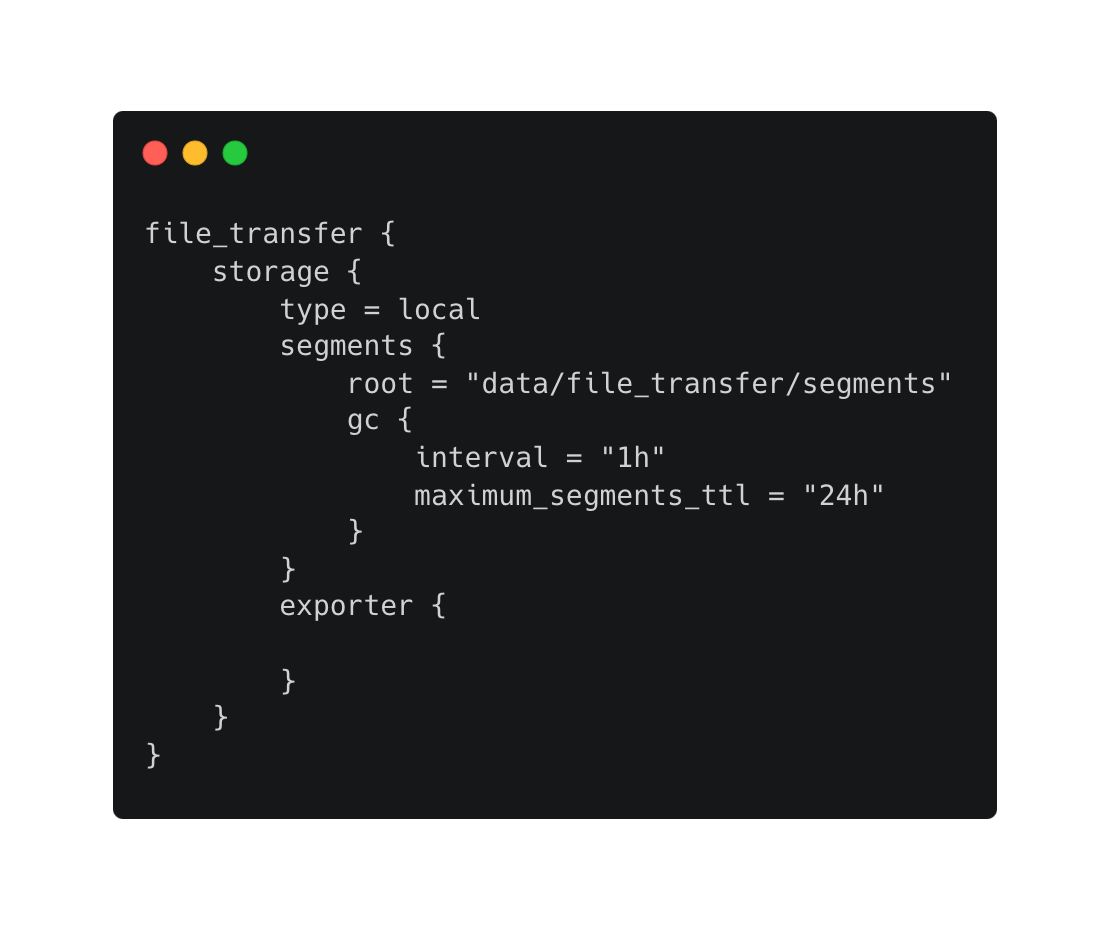
\includegraphics[width=7cm, keepaspectratio]{images/ft_storage_fs_conf.png}
    \end{center}
\end{frame}


\begin{frame}
    \frametitle{File Transfer}
    \framesubtitle{emqx\_ft\_storage\_exporter}

    \begin{center}
        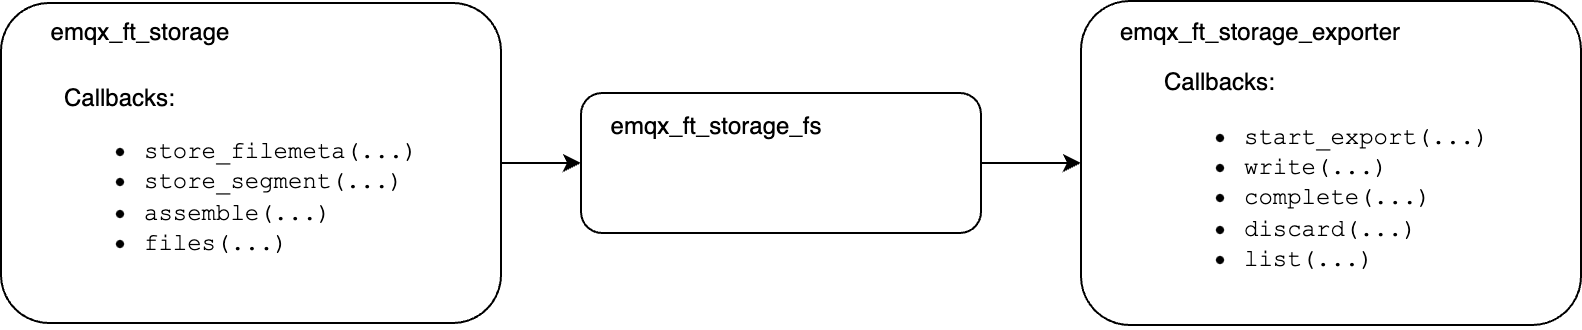
\includegraphics[width=9cm, keepaspectratio]{images/ft_storage_fs.png}
    \end{center}
\end{frame}


\begin{frame}
    \frametitle{File Transfer}
    \framesubtitle{emqx\_ft\_storage\_exporter}

    \begin{center}
        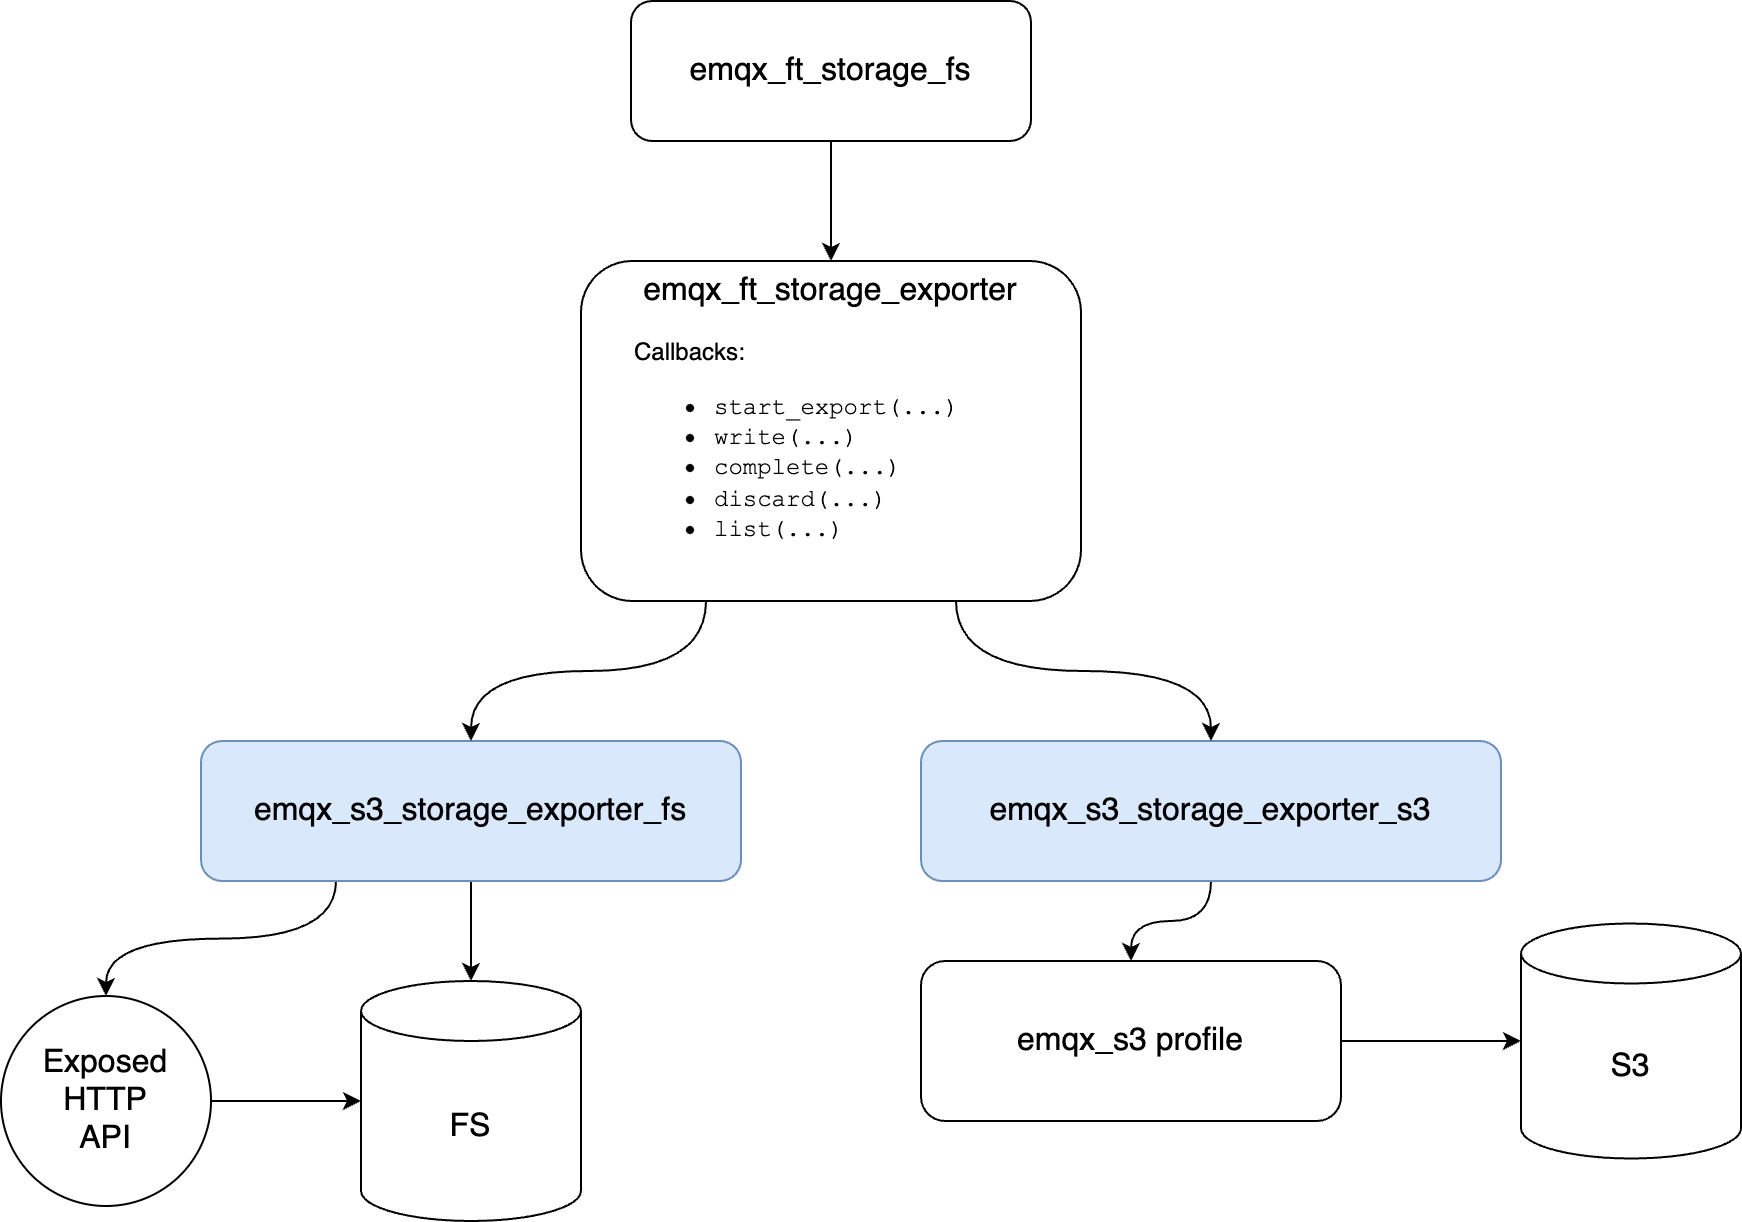
\includegraphics[height=5cm, keepaspectratio]{images/ft_storage_fs_exports.png}
    \end{center}
\end{frame}

\begin{frame}
    \frametitle{File Transfer}
    \framesubtitle{emqx\_ft\_storage\_exporter\_fs}
    \begin{itemize}
        \item Exports ready files to the local file system
        \item Saves metadata in the local file system together with the file
        \item Uses some bucketing logic to avoid having too many files in one directory
        \item Exposes its own API to access exported files
    \end{itemize}
    \begin{center}
    \end{center}
\end{frame}

\begin{frame}
    \frametitle{File Transfer}
    \framesubtitle{emqx\_ft\_storage\_exporter\_fs file structure}

    \begin{center}
        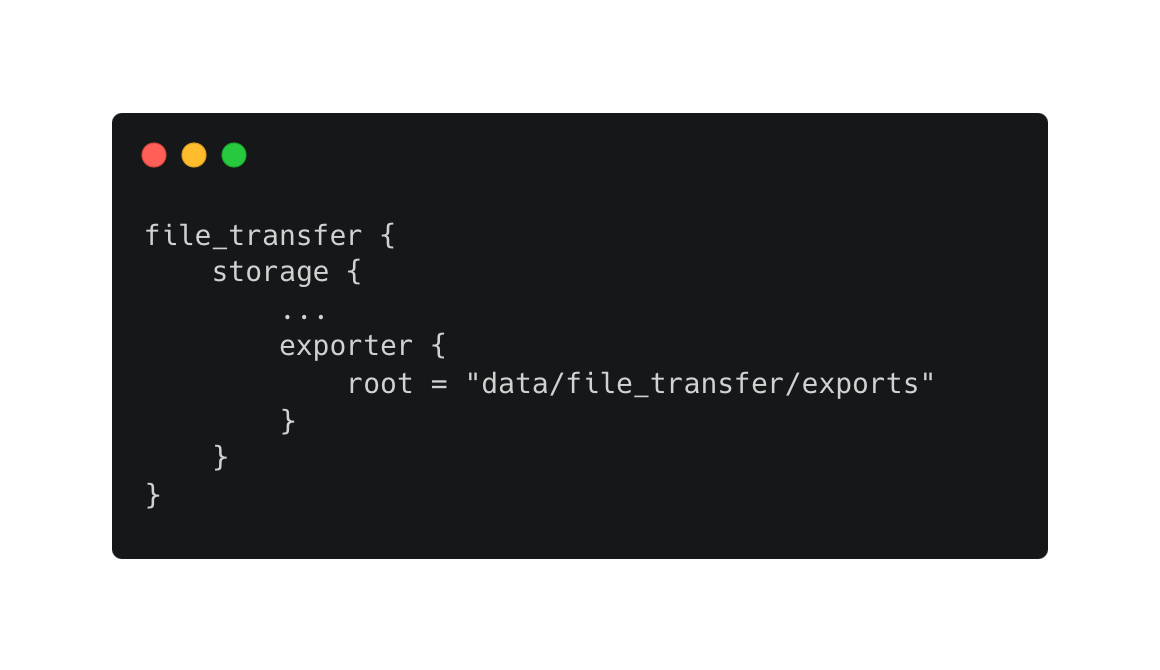
\includegraphics[width=9cm, keepaspectratio]{images/ft_storage_fs_exports_fs_conf.png}
    \end{center}
\end{frame}

\begin{frame}
    \frametitle{File Transfer}
    \framesubtitle{emqx\_ft\_storage\_exporter\_fs config}

    \begin{center}
        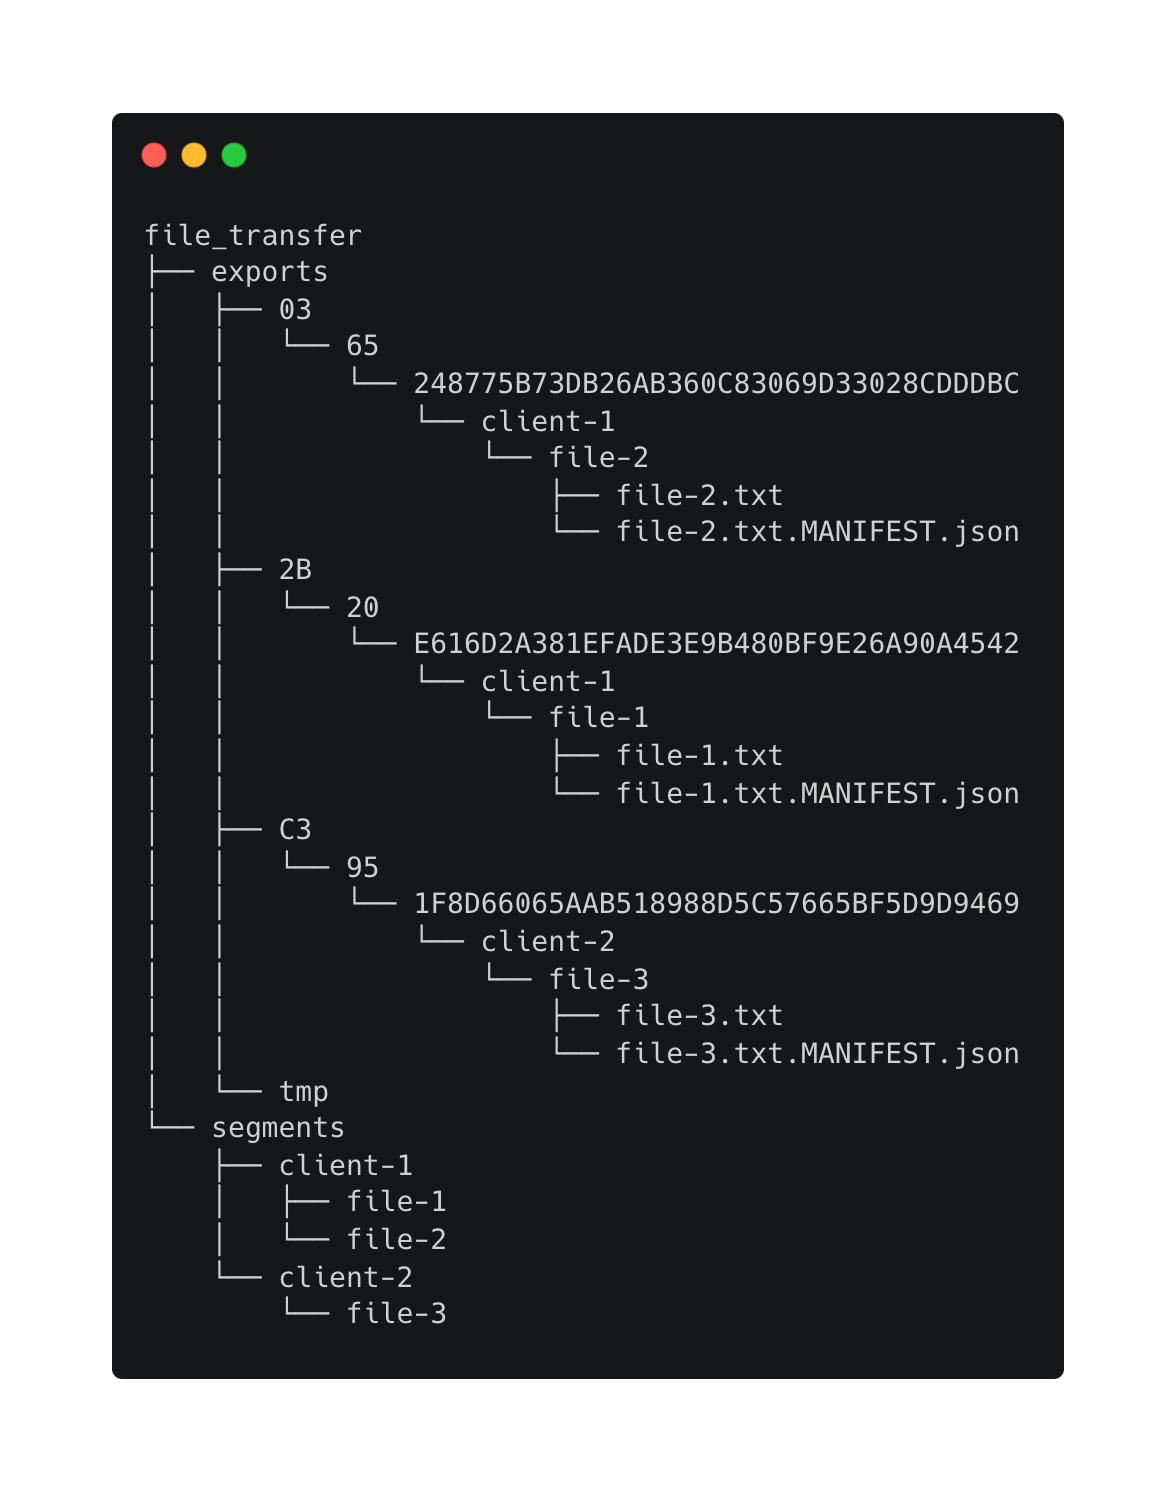
\includegraphics[height=7cm, keepaspectratio]{images/ft_storage_fs_exports_fs_tree.png}
    \end{center}
\end{frame}


\begin{frame}
    \frametitle{File Transfer}
    \framesubtitle{emqx\_ft\_storage\_exporter\_s3}
    \begin{itemize}
        \item Exports ready files to S3 compatible storage
        \item Saves metadata as S3 object metadata
        \item Quite a thin wrapper around \lstinline{emqx_s3} application
        \item Does not expose its own API for file access
    \end{itemize}
    \begin{center}
    \end{center}
\end{frame}

\begin{frame}
    \frametitle{File Transfer}
    \framesubtitle{S3 Constraints}
    \begin{itemize}
        \item Standalone application, not related to File Transfer
        \item Simply reusable \& pluggable
        \item * Not strongly coupled with the underlying HTTP library (we use \lstinline{ehttpc})
        \item * Supporting long living interactions with S3 (e.g. multipart upload)
    \end{itemize}
    \begin{center}
    \end{center}
\end{frame}

\begin{frame}
    \frametitle{File Transfer}
    \framesubtitle{emqx\_ft\_storage\_exporter\_s3 config}

    \begin{center}
        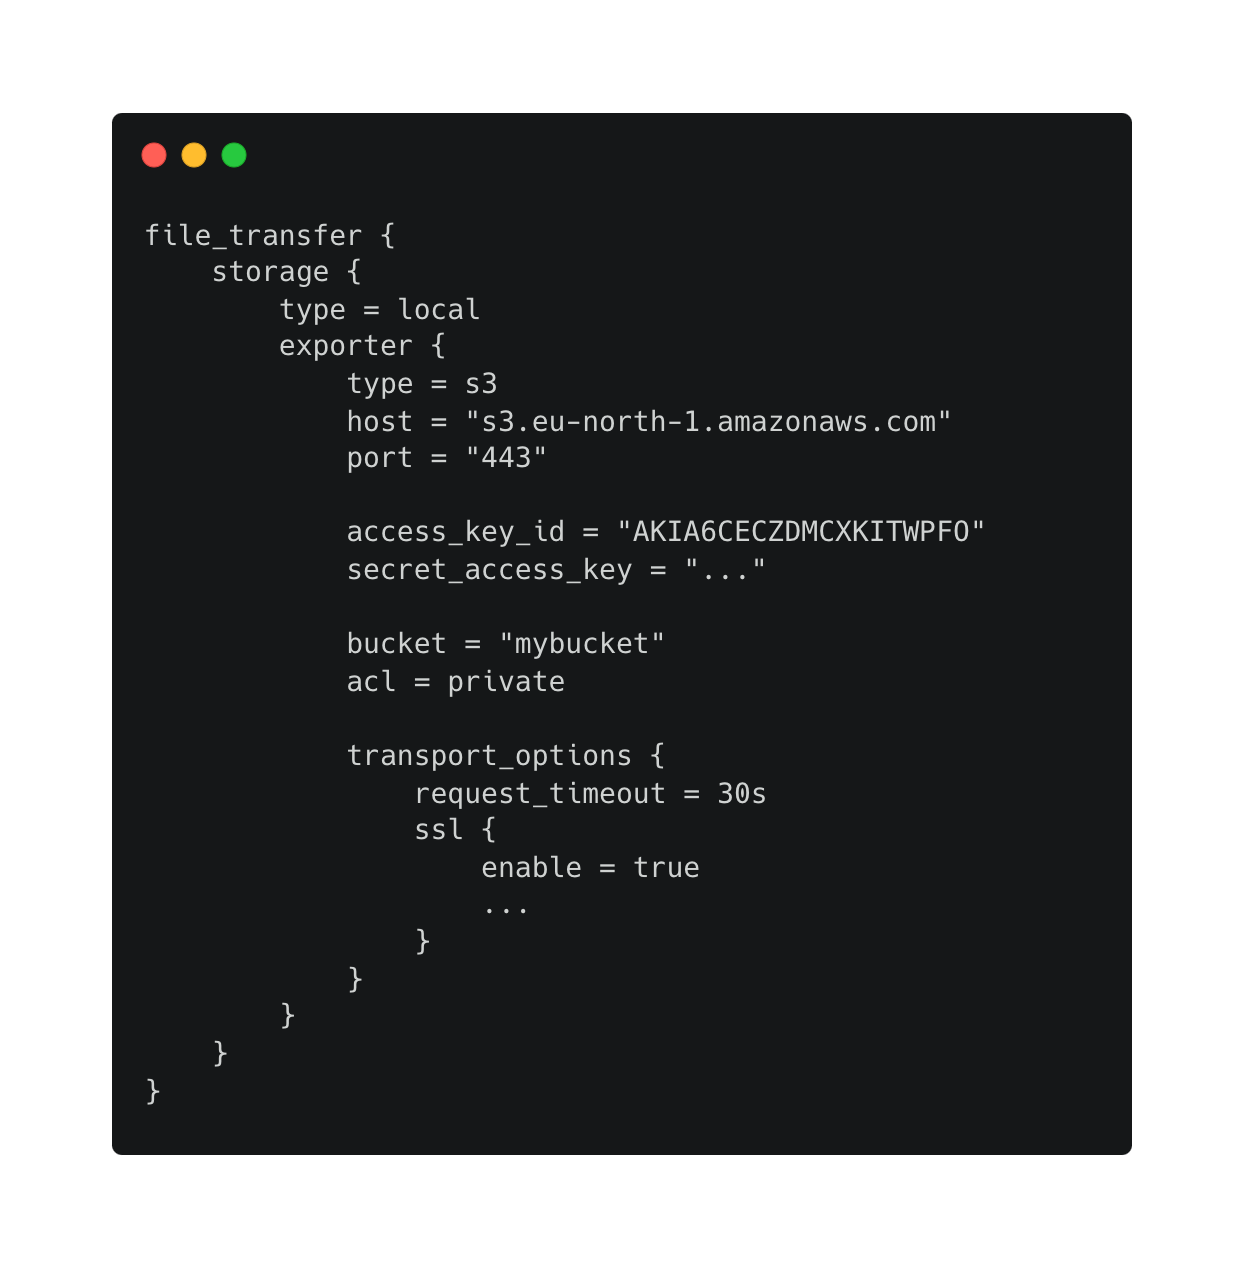
\includegraphics[height=7cm, keepaspectratio]{images/ft_storage_fs_exports_s3_conf.png}
    \end{center}
\end{frame}

\begin{frame}
    \begin{center}
        Thank you!
    \end{center}
\end{frame}

\end{document}
